\chapter{Multiobjective optimization}
\label{chap:Multi-objective}
%\begin{refsection}
%\glsresetall
\abstract{Before tackling the problem of multiple criteria for \gls{pid} tuning, the multi-objective optimization is explained in general. First the basic formulation of the optimization problem is presented with the introduction of the Pareto front concept. The methodology chosen to solve the multiobjective optimization problem is to transform the multi-criteria situation into a single scalar cost function. However it is known that this scalarization procedure may not yield to a good Pareto front. For this reason several scalarization methods are presented and compared. The Pareto found using this scalarization methods may be used as just data that can be later used or may be directly used as part of a decision tool useful to select the final solution to the problem.} 

\section{Formalization of the multiobjective optimization problem}
\label{sec:MOOPForm}
%
A \gls{moop} arises when, in order to solve a given problem or design, it is necessary to optimize several cost functions at the same time. 

In general, these cost functions depend on the same variables and usually are in conflict.  In addition, they may be independent of one another, that is, the value of the variables that optimize one of the function do not necessarily optimize the other cost functions.

In those cases, given a set of cost functions:
\begin{equation}
\mathbf{F}(\xv)=\left[F_1(\xv), F_2(\xv), F_3(\xv), \ldots, F_k(\xv)\right]^T
\label{eq:functions}
\end{equation}
%
that depends on $n$ different variables $\xv=\left[x_1, x_2, \ldots, x_n \right]^T$, $\xv \in \mathbf{X}$, where $\mathbf{X}$ is the feasible decision space. The \gls{moop} may be formulated as follows \citep{Marler2004}:%
%
\begin{subequations}%
	\begin{align}%
	&\min_\xv \mathbf{F}(\xv), \label{eq:Min01}\\ %
	&\text{s.t.}\nonumber\\%
	& \hspace{5mm} g_j(\xv) \leq 0, \qquad j=1,2,\ldots,m  \label{eq:Min02}\\ %
	& \hspace{5mm} h_l(\xv) = 0, \qquad l=1,2,\ldots,e  \label{eq:Min03}%
	\end{align}%
	\label{eq:OptProb}%
\end{subequations}%
%
where $g_j(\xv)$ is the $j$-th inequality constraint and $h_l(\xv)$ is the $l$-th equality constraint. 
%
\subsection{Definition of the Pareto front}
In general, it is not possible to find a set of variables values that simultaneously minimizes all $F$ functions. In fact, the optimization problem in \eqref{eq:OptProb} have multiple equally optimal solutions in the sense of the Pareto optimality. According to \citet{Marler2004}:
\begin{quote}
	``A point $\xv^*\in \mathbf{X}$, is Pareto optimal iff there does not exist another point, $\xv \in \mathbf{X}$, such that $\mathbf{F}(\xv)\leq\mathbf{F}(\xv^*)$, and $F_i(\xv)<F_i(\xv^*)$ for at least one function''
\end{quote}

The concept of Pareto optimality is represented in %
%
\begin{figure}[tb]
	\centering
	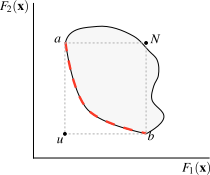
\includegraphics[width=0.8\columnwidth]{Ch5planoFun01}
	\caption{All possible solutions and the Pareto front in the function space.}
	\label{fig:planoFun01}
\end{figure}
%
figure~\ref{fig:planoFun01} for a two-function multi-objective optimization. The gray area represents the feasible function space, given by the value of $F_1(\xv)$ and $F_2(\xv)$ for all $\xv \in \mathbf{X}$. From all those points, only the points in the curve from ``a'' to ``b'' (marked with a thicker dash line) are Pareto optimal because there is not another point in the feasible decision space with a lower value of $\mathbf{F}$, but there is at least one point that has a lower value for either $F_1$ or $F_2$. The curve from ``a'' to ``b'' is the Pareto front and contains all possible solutions to problem \eqref{eq:OptProb} that are Pareto optimal. These solutions are always in the edge of the feasible function space, closer to the utopia point (the ``u'' point in the figure). The utopia point is a point in the space where all the cost functions have their minimum value. As it can be seen from figure~\ref{fig:planoFun01}, this point is more likely to be outside of the feasible function space.

Points ``a'' and ``b'' are called anchor points and represent the combination of decision variables that optimizes at least one of the functions. In this case, ``a'' is the point where function $F_1(\xv)$ has its minimum value whereas ``b'' the one in which $F_2(\xv)$ has its minimum value.

Point ``N'' is called the pseudo-nadir point, and is defined as the point with the worst values of all the anchor points.

\subsection{Practical example}
\label{sec:ParetoPractical}
To get an insight of the concept of Pareto Front, an industrial controlled process will be considered. In this particular case, the relationship between \gls{tv} and \gls{iae} for the controller as regulator is studied. However, in the rest of the book, the compromises between the response for different sources of disturbances will be considered. The objective of this section is to show that the concept of Pareto front can be used with diverse cost functions.

In Section~\ref{sec:ParetoApproach}, different approaches to obtain the Pareto are presented. For this particular example a ``brute force'' approach is taken. The process that is used as example is a \gls{wwtp}.

The residual water after it has been used in residential commercial or industrial zones is known as wastewater. It is collected through sewers with the intention to be treated to be later deposited in receiving waters like rivers, lakes or the sea. According to \citet{Olsson1999} ``while the primary goal of a treatment plant is to achieve an average reduction in nutrient levels, the secondary goal is disturbance rejection, to achieve good effluent quality in spite of the many disturbances''. One of the characteristics of this process is that it is subject to large variation in the influent characteristics like the substrate concentration, oxygen levels and even flow. For example in \citet{Henze1997}, it is shown an example were the influent flow at midday can reach up to 244\% of the average flow in one day, while minimum could reach 32\% of the average flow.

To reduce the substrate levels, the idea is to stimulate the grow of microorganism that consume the substrate, to later be removed in the settler. This biological process is known as Activated Sludge Process (ASP) and it is one of the most important methods for wastewater treatment \citep{Henze1997}. Bacteria is the most important component of the sludge. These bacteria can remove carbon components and also nitrogenous components from the influent. To control the grow of bacteria, air is pumped into the wastewater while being store in tanks.

As pointed out by \citet{Jeppsson1996}, from the point of view of the bacteria, the organic particles in the influent are used as its source of energy. Bacteria take the oxygen and the particles and produce other simpler compounds (methane for example). The air injected in the tanks is its main source of oxygen and therefore is the principal manipulated variable of the system. However it is common to also have anoxic tanks (that is, tanks without external oxygen) that are used to promote the growth of bacteria that takes the oxygen directly from the water in the tank. Anoxic tanks are used to remove the nitrogenous components. The suspended material, the sludge, is remove from the water by settlers. Part of the sludge is recirculated to the system in order to keep enough biomass in the tanks, while the rest is dispose out of the loop to be used as fertilizer.

Therefore, the basic layout of a \gls{wwtp} using the ASP contains an aeration tank and a settling tank as represented in 
as presented in %
%
\begin{figure}[tb]
	\centering
	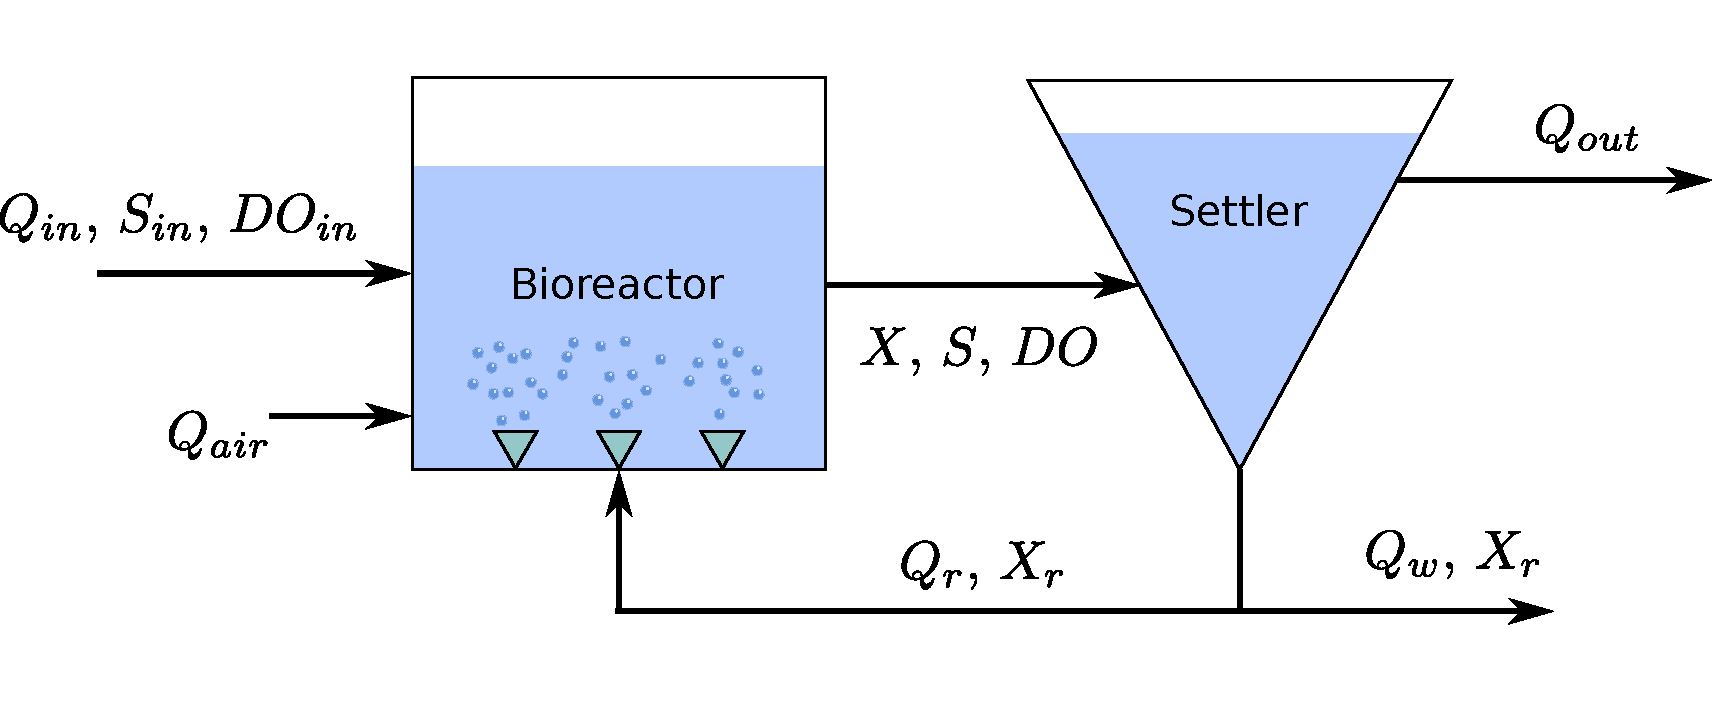
\includegraphics[width=\linewidth]{Ch5WTP}
	\caption{Representation of a simple wastewater treatment process.}
	\label{sec:Ch5WTP}
\end{figure}
%
Figure~\ref{sec:Ch5WTP}. The ``cleaned'' water is withdrawn from the top of the settler while part of the sludge is recirculated to the bioreactor and the rest is used to produce where the treated wastewater is deposited in the receiving water while a concentrated sludge is withdrawn from the bottom \citep{Henze1997}. This concentrated sludge can be recycled in order to maintain a high density of biomass in the thanks.

One of the characteristics of \gls{wwtp}s is their high energy consumption \citep{Longo2016}. The bioreactor needs electricity to produce the aeration, move the water using pumps and continuous stirring. At the same time it is necessary to cope with disturbances coming from the influent. With this train of logic, from a control perspective, it is necessary to keep the system regulated, at the same time that the energy is minimized.

In order to frame this problem mathematically, first a model has to be selected. In this case, the model first proposed in \cite{Nejjari1999} and slightly modified in \cite{Han2008} will be considered. This model is a fourth order non-linear set of equations found after a material balance is performed. The model is given by:
\begin{equation}
	\begin{split}
	\frac{d X (t)}{dt} &= \mu(t) X(t) - D(t) (1+r)X(t)+rD(t)X_r(t)\\
	\frac{d S (t)}{dt} &= -\frac{\mu(t)}{Y}X(t) - D(t)(1+r)S(t)+D(t)S_{in}(t)\\
	\frac{d DO (t)}{dt} &= - \frac{K_0 \mu(t) X(t)}{Y} - D(t)(1+r)DO(t)\\
					& \qquad + \alpha Q_{air}(t) \left(DO_{max} - DO(t)\right) +D(t) DO_{in}(t)\\
	\frac{d X_r (t)}{dt} &= D(t) (1+r) X(t)- D(t) \left( \beta + r \right) X_r(t)\\
	%
	\mu(t) &= \mu_{max} \frac{S(t)}{K_S + S(t)} \cdot \frac{DO(t)}{K_{DO}+DO(t)}
	\end{split}
	\label{frac:WWTPModel}
\end{equation}
%
where,
\begin{itemize}
	\item $X(t)$ is the biomass concentration
	\item $S(t)$ is the substrate concentration
	\item $DO(t)$ is the dissolved oxygen in the bioreactor
	\item $X_r(t)$ is the recycled biomass concentration
	\item $D(t)$ is the dilution rate
	\item $DO_{in}(t)$ is dissolved oxygen concentration in the influent
	\item $Q_{air}(t)$ is the aeration rate
	\item $\mu(t)$ biomass growth rate
\end{itemize}
%
and the parameters are:
\begin{itemize}
	\item $DO_{max}$ is the maximum dissolved oxygen concentration
	\item $S_{in}$ is the substrate concentration in the influent
	\item $Y$ is the biomass yield factor
	\item $\mu_{max}$ is the maximum specific growth rate
	\item $K_S$ is the affinity constant
	\item $K_{DO}$ is the saturation constant
	\item $\alpha$ is the oxygen transfer rate
	\item $K_0$ is a model constant
	\item $r$ is the recycled sludge rate
	\item $\beta$ is the removed sludge rate
\end{itemize}

The values of all the parameters are given in %
\begin{table}[tb]
	\centering
	\caption{Parameter values for the WWTP model}
	\begin{tabular}{lll}
		\toprule
		$DO_{max} = \SI{10}{\milli\gram\per\liter}$ & $S_{in} = \SI{200}{\milli\gram\per\liter}$ & $DO_{in} = \SI{0.5}{\milli\gram\per\liter}$\\
		$Y = 0.65$ & $\mu_{max} = \SI{0.15}{\milli\gram\per\liter}$ & $r = 0.6$ \\
		$K_S = \SI{100}{\milli\gram\per\liter}$ & $K_{DO} = \SI{2}{\milli\gram\per\liter}$ & $\alpha = 0.018$ \\
		$K_0 = 0.5$ & $\beta = 0.2$\\
		\bottomrule
	\end{tabular}
	\label{tab:ParamValues}
\end{table}
%
Table~\ref{tab:ParamValues}, while the value of the variables in the selected operation point is given in %
%
\begin{table}[tb]
	\centering
	\caption{Variables values for WWTP in operation point}
	\begin{tabular}{ll}
		\toprule
		$Q_{air0} = 27.57$ & $D_0 =  0.025$ \\
		$S_{in0} = \SI{200}{\milli\gram\per\liter}$ & $DO_{in0} = \SI{0.5}{\milli\gram\per\liter}$\\
		$X_0 = 298.24$ & $S0 = 10.29$\\
		$DO_0 = 5.00$ & $X_{r0} = 596.47$\\
		\bottomrule
	\end{tabular}
	\label{tab:WTPOP}
\end{table}
%
Table~\ref{tab:WTPOP}.

The idea is to study the relationship between the \gls{iae} for the closed-loop regulation against the dilution rate disturbances and the \gls{tv} of the aeration rate. The \gls{iae} represents the performance of the plant while the \gls{tv} is an indirect measure of the energy required to accomplished that level of performance. It is expected that a good disturbance rejection response (lower \gls{iae}) implies a higher \gls{tv} (which means a more aggressive control signal).

The closed-loop is controlled by means of a \gls{pi} controller that manipulates the aeration rate in order to keep the dissolved oxygen concentration in the reactor around $5.0$ in the presence of dilution rate disturbances. The model was implemented with an S-function and the simulations were performed using \simulink. The implementation of the model can be found in the software companion to this book and is represented in Figure~\ref{fig:Ch5SimulinkWTPModel}. The parameters of the \gls{wwtp} can be varied by means of a mask, as presented in Figure~\ref{fig:Ch5WTPMask}. The parameters and the initial conditions can be set manually, alternatively, an initialization script is also included, with the parameter and variables values presented in Table~\ref{tab:ParamValues} and Table~\ref{tab:WTPOP}.
%
\begin{figure}[tb]
	\centering
	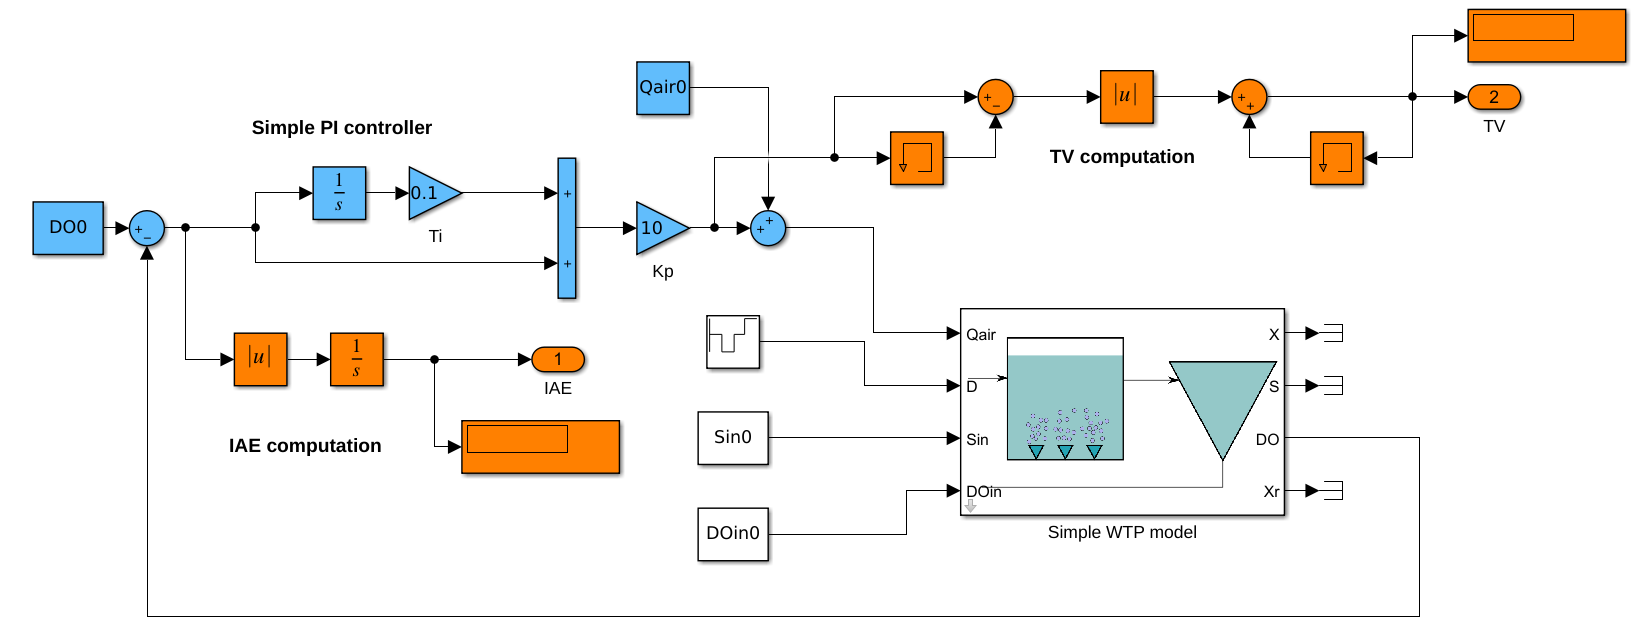
\includegraphics[width=\linewidth]{Ch5SimulinkWTPModel}
	\caption{\simulink implementation of the \gls{wwtp} control system.}
	\label{fig:Ch5SimulinkWTPModel}
\end{figure}
%
\begin{figure}[tb]
	\centering
	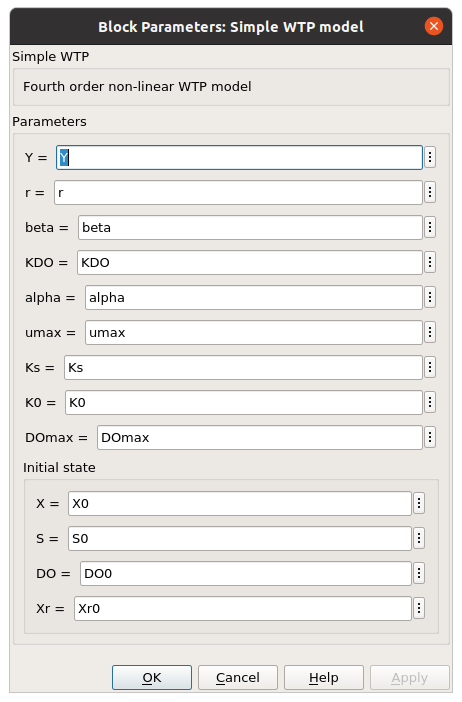
\includegraphics[width=0.4\linewidth]{Ch5WTPMask}
	\caption{Mask that allows the parameters of the \gls{wwtp} model to be changed.}
	\label{fig:Ch5WTPMask}
\end{figure}

The implementation of the controller is very simple, a more complete version is used in Section~\ref{sec:CSTRVandeVusse}, where a chemical process is used to show the multivariable approach presented in this book. The \gls{iae} and \gls{tv} values are also computed within the \simulink{} model.

In Section~\ref{sec:ParetoApproach}, some methods to generate the front are presented, however, for this practical example, a more basic approach is taken. The idea can be summarized as follows: Varying the values of $K_p$ and $T_i$ within a certain range, compute both \gls{iae} and \gls{tv} for all possible combinations. From this data, found the Pareto front.

This procedure is simple, however it is necessary to do a simulation of the system for every point, as presented in Figure~\ref{fig:Ch5ParetoWTP}. %
\begin{figure}
	\centering
	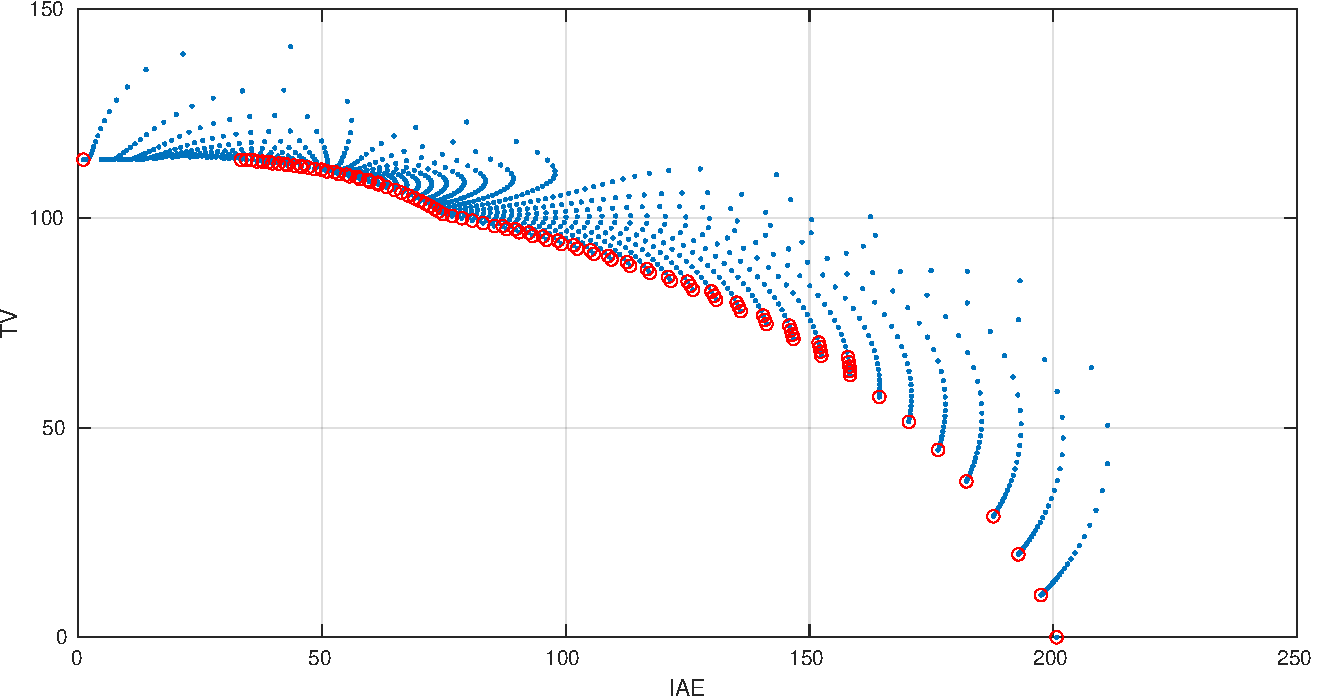
\includegraphics[width=\linewidth]{Ch5ParetoWTP}
	\caption{Result of the simulation for \gls{wwtp} considering \gls{iae} and \gls{tv}.}
	\label{fig:Ch5ParetoWTP}
\end{figure}
%
This figure represents 2500 simulations where the resulting \gls{iae} and \gls{tv} are represented in the plane known as the function space. One expect the Pareto to be shaped like the example presented in Figure~\ref{fig:planoFun01}, however this is not necessarily true for all cases, as can be verified with this particular example. Nevertheless, the Pareto arises once all the simulations are completed. All points represent a particular set of values of $K_p$ and $T_i$. The points marked with a circle are the ones that belong to the Pareto. All these points represent optimal values of $K_p$ and $T_i$ because, it is not possible to find any other solution capable to have a lower value for one of the functions without worsening the other function.

For this particular example, the left anchor point (the one with lower value of \gls{iae}) can be considered as the case with the controller with the best performance but with a higher consumption of energy. Since there are some points above this point, it can be said that there are more costly controllers but with worst performance. It is obvious that this set of controllers are not of our interest, that is the dominated solution can be disregarded.

On the other side, the anchor point on the right (the one with lower \gls{tv}) is an interesting case, in which the controller is set in open loop (the value of $K_p$ is equal to zero). The particular value of \gls{iae} for this case is totally dependent of the disturbance signal used for the simulation. However the behavior found in this example is what would be expected: better performance implies a more aggressive control signal.

However, it is clear that is not efficient to find the Pareto front using brute force. Consider that, from all the points computed, only a small fraction ($8.4\%$ to be exact) correspond to cases in the front. A lot of computer power was literally wasted. Also, note that, by varying $K_p$ and $T_i$ evenly, it was not possible to found an evenly distributed front. It is also important to note that not all points that were selected as part of the Pareto may not actually belong to it. If more points were found, it may be possible to find a better representation of the front but the computation needed (an the time) will not be productive.

However, once the Pareto is obtained, the user is capable to make decisions regarding the final selection of the parameters. For example, the decision maker can allow a level of degradation in \gls{iae} to obtain certain improvement on the \gls{tv}. Let's define the \gls{iae} degradation $\alpha_{iae}$ as:
\begin{equation*}
	\alpha_{IAE} = \frac{IAE - IAE_{min}}{IAE_{max}-IAE_{min}},
\end{equation*}
%
with such definition, a value of $\alpha_{IAE} = 0$ represents zero degradation, that is, the case where the $IAE$ value is at its minimum. On the other hand, a value of $\alpha_{IAE} = 1$ represents the maximum value of \gls{iae} within the Pareto front, that is, the maximum possible degradation.

With this in mind and looking at the Pareto in Figure~\ref{fig:Ch5ParetoWTP}, it is clear that, to obtain an improvement on \gls{tv} of about $20\%$, it is necessary to degrade the \gls{iae} about $50\%$. This may or may not be appropriate for the application. But, whichever point the decision maker takes as the final controller, if it is one of the points in the front, he or she can be sure that it is optimal.

But the efforts should be directed to find the Pareto from the beginning, not as a subproduct of a brute force task. Now, certain techniques are shown that are intended to directly find the best representation of the Pareto with as little effort as possible. Later in the book, some tools are proposed to take advantage from the Pareto, once it has been found.

\subsection{Different approaches to obtain the Pareto front}
\label{sec:ParetoApproach}
In its most basic form, the Pareto front is found by performing several optimizations, each of which are computed by varying some kind of parameters. Because of this, the idea is to be able to use standard optimization methods to find each point of the Pareto. However, this standard methods are meant to solve single objective problems.

As for single objective optimization there is two big families of methods to solve the problem: Bio-inspired methods that use some kind of heuristic in order to find the minimum of the cost function and deterministic methods mostly based on certain gradient of the function.

In this section, a short review on both families is presented. However, because of the deterministic nature of the gradient based methods, in this book the later family is chosen tool for solving \gls{moop}.

In \citet{Zhou2011} a review on multi-objective evolutionary algorithm is presented. The author indicates that several of the algorithms are similar to the non-dominated sorting genetic algorithm II (NSGA-II) \citep{Deb2002}. Genetic algorithms are based in the idea of random mutation across generations and interchange of genes from parents to children. They also explain other kind of algorithms like particle swarm optimization which is based on the social behavior of bird flocking or fish schooling \citep{Eberhart1995}. Originally this method was employed for single function optimization, but it has been extended for multiple cost functions. Other methods that has been used for solving \gls{moop}, have a probabilistic nature like Ant Colony Optimization \citep{Dorigo2005} or the Cross Entropy method \citep{Rubinstein2004}. One drawback is that these methods are heuristic, and may yield different results each time they are computed. However, the main advantage is that they probably are able to find the global minimum of the functions.

Specifically, for \gls{pid} control, evolutionary algorithms have been used in \citet{Reynoso-Meza2012b} for the multivariate process of the Wood and Berry distillation column. Another case is presented in \citet{Pierezan2014} where multi-objective Particle Swarm Optimization is applied on multivariable PID controllers tuning to improve the performance of a robotic manipulator. This method was also used in \citet{Tian2014} but applied to a nonlinear process continuous stirred tank reactor. Also in \citet{Mahdavian2014}, a multi-objective optimization for \gls{pid} control of a greenhouse electrical lighting system based on the cost of electricity is investigated and solved using an evolutionary algorithm. Multiobjective salp swarm algorithm (MSSA) with opposition based learning initialization and evolution was used in \citet{Domingues2019} for tuning the parameters of a \gls{pid} controller for an Antilock Braking Systems with good results over NSGA-II, but the later was more consistent with the results.

\subsubsection{Comparison of bioinspired methods for process control}
%
Now lets compare how is the performance of some bioinspired methods for industrial process control. In \citet{Cespedes2016} Ant Colony Optimization, Invasive Weed Colony Optimization \citep{Mehrabian2006}, Linear Biogeography-based optimization \citep{Simon2008}, Genetic Algorithms and Particle swarm optimization are compared when solving the tuning of an industrial \gls{pid} controller for \gls{soptd} plants. The main results are summarized below. These methods were used to minimize $J_{di}$, but it is important to note that, for this particular study, the methods were not implemented to produce a Pareto front (i.e. to minimize $J_r$ at the same time). The idea is just to compare different bioinspired methods computationally. However, they can be adapted to be used in multiobjective optimization problems with small changes.

\paragraph{Ant Colony Optimization}
\label{sec:ACO}
Ants can naturally fin the shortest path between its nest and the food source by producing some kind of chemical signaling that let the complete population know the path that most ants are using.  As pointed by \citet{Dorigo2006}: ``these  ants  deposit pheromone  on  the  ground  in  order  to  mark  some  favorable path that should be followed by other members of the colony. Ant colony optimization (ACO) exploits a similar mechanism for solving optimization problems''

Initially a fixed number of ``artificial ants'' are assigned a given random path which represent the different values of the decision variables that minimize some cost function. The quantity of ``artificial pheromone'' is also assigned to each path according to the fitness of the solution. The algorithm then start to discard some paths and in the end, the path with more ``pheromone'' is supposed to represent the optimal solution \citep{Goss1989}.
%
\paragraph{Invasive Weed Colony Optimization}
\label{sec:IWO}
%
Invasive Weed Optimization (IWO) is a search algorithm first presented in \citet{Mehrabian2006a}. The idea behind the method is based on how weed colonize and distribute the space around \citep{Binitha2012}. IWO can solve multidimensional optimization problems following the next steps:
%
\begin{enumerate}
	\item Initialize the population: First a set of random initial solutions widespread over the multidimensional problem space are selected. These solution are considered as members of the weed colony. %, this random population based on VarMin, VarMax and VarSize.
	%%
	\item Reproduction: Each member of the population is allowed to produce seeds depending on its own, as well as the colony's, lowest and highest fitness, such that, the number of seeds produced by a weed increases linearly from lowest possible seed for a weed with worst fitness to the maximum number of seeds for a plant with best fitness (which corresponds to the lowest objective function value for a minimization problem)\citep{Kundu2011}%
	%%
	\item Spatial dispersal: The seeds are distributed randomly across the search space with a varying variance. The idea behind this is that the seeds will not be near (that is, be similar) to the parent plant.
	%
	\item Competitive exclusion: When all seeds have a defined position, they are ranked using the cost function to minimize. The weeds with lower function value are discarded, since this cost function is considered to represent the fitness of each plant, when discarding the ones with worst value, it is ensure that only the specimens with better fitness survive and are able to reproduce in the next generation.
\end{enumerate}
%
\paragraph{Linear Biogeography-based optimization}
In its original form, Biogeography is the branch of biology that studies the geographical distribution of plants and animal and the mathematical models associated with the extinction and migration of species \citep{MacArthur1967}.

Biogeography-based optimization (BBO) is an evolutionary algorithm in which each possible solution to the problem is treated as an habitat (or island). The solution with a better cost function then is considered to be a better habitat  because the value of the solution is analogous to the characteristics of the habitat that let different species to thrive \citep{Simon2008}.

Good habitats are considered to have high rate of emigration, because its good features allows an increase in the number of species. This increase may lead to a saturation in its capacity to house more species. The solutions with lower fitness has a high rate of immigration, because animals and plants search for less concentrated habitats to grow and reproduce.

New solutions are found by mixing the characteristics of each habitats according to its emigration and immigration rates. Then, this new habitats are compared against each other, and the best ones are used to form new solutions until an optimal is found.

\paragraph{Genetic Algorithms}
The Genetic Algorithms (GA) are based on the ideas of evolution, genetics and natural selection. The main characteristics of GA are~\citep{Simon2013}:
%
\begin{itemize}
	\item It tries to simulate the sexual reproduction of a biological population.
	\item The individuals have a finite life span.
	\item In each generation, some new characteristics of the population arises due to random mutation.
	\item There is a positive correlation between the ability to survive and the ability to reproduce.
\end{itemize}

As in nature, the idea behind GA is that only the best fitted specimen in a population are able to reproduce, and therefore, pass it genome to the next generation. This ``fitness'' value is considered to be the cost function that is intended to be minimized \citep{Mitchell1995}.

In this case, each individual is viewed as a possible solution to the problem. Its value is coded as a binary chain, simulating the genetic information of living beings. The algorithm then decides which individuals of each generation are allowed to reproduced and therefore, only the ones with a minimal the minimal cost function survive.
%
\paragraph{Particle swarm optimization}
Particle swarm optimization (PSO) is also a search algorithm. But in this case, each solution in the pool of initial solutions are considered to represent an individual in a swarm (for example a flock of birds). In general, each individual is called a particle which represents a possible solution to the problem.The interesting characteristic of this method is that the adjustment of each particle depends on its history and its relationship with the neighboring particles~\citep{Shi2004}.

If for example, a flock of birds is considered as the biological counterpart, the objective is to define an algorithm that mimics the movement of this flock that naturally occurs without an apparent leader, this phenomenon is usually called swarm intelligence~\citep{Kennedy1995}. At each iteration, the acceleration of each particle is changed to move them to the best solutions found.

\paragraph{Comparison of each method for industrial controller tuning}
%
In this comparison a \gls{pid} controller is tuned as regulator using the methods presented above, for a second order overdamped system with pure time delay. The results of each method were obtained with a computer equipped with an Intel Core i5-3470 CPU at 3.20GHz and 8 GB of RAM using \matlab as programming language.

For comparison purposes, the result of the optimization using the interior-point (IP) algorithm is presented. In all cases it was required that at least 125 iteration where performed in order to let all methods to explore the complete solution space. Also, in al cases, the initial solutions where selected around the same point. A total of 100 different experiments were applied to 9 different plants. The difference in the plants were the time delay and the relationship between the larger and smaller time constant. This plants are presented in %
%
\begin{table}[tb]%
	\centering
	\caption{Parameter of the test plants.}
	\label{tab:Plants}
	\begin{tabular}{cc}
		\toprule
		Plant & Parameters \{$K$, $T$, $L$, $a$\}\\
		\midrule
		P1 & \{1, 1, 0.1, 0.0\}\\
		P2 & \{1, 1, 0.1, 0.5\}\\
		P3 & \{1, 1, 0.1, 1.0\}\\
		P4 & \{1, 1, 1.0, 0.0\}\\
		P5 & \{1, 1, 1.0, 0.5\}\\
		P6 & \{1, 1, 1.0, 1.0\}\\
		P7 & \{1, 1, 2.0, 0.0\}\\
		P8 & \{1, 1, 2.0, 0.5\}\\
		P9 & \{1, 1, 2.0, 1.0\}\\
		\bottomrule
	\end{tabular}
\end{table}
%
Table~\ref{tab:Plants}. It has to be noticed in these plants that they cover all the spectrum of plants, from plats with small time delay ($L=0.1$) to plants where the time delay is twice the value of the larger time constant.

It was found that all method were able to find and optimal similar to the one found using the deterministic method IP. When comparing the disturbance rejection response, presented in %
%
\begin{figure}[tb]%
	\centering
	\begin{tikzpicture}
	\begin{axis}[
	xlabel={time (s)},
	ylabel={amplitude},
	legend pos=north east,
	legend style = {font=\scriptsize},
	grid=major,
	xtick={0,2,...,20},
	xmin=0,
	xmax=20,
	]
	\addplot+[mark=none] table[x=time, y=ACO, col sep=comma]{./tablas/ComparacionJdi.csv};
	\addplot+[mark=none,dashed] table[x=time, y=IWO, col sep=comma]{./tablas/ComparacionJdi.csv};
	\addplot+[mark=none,dashdotted] table[x=time, y=LBBO, col sep=comma]{./tablas/ComparacionJdi.csv};
	\addplot+[mark=none,dashdotdotted] table[x=time, y=GA, col sep=comma]{./tablas/ComparacionJdi.csv};
	\addplot+[mark=none,loosely dashdotdotted] table[x=time, y=PSO, col sep=comma]{./tablas/ComparacionJdi.csv};
	\legend{{ACO, IAE=1.6718},{IWO, IAE=1.273},{LBBO, IAE=1.6167},{GA, IAE=1.2934},{PSO, IAE=1.2729}}
	\end{axis}
	\end{tikzpicture}
	\caption{Simulation of the different bio-inspired optimization methods to an unitary step change in the disturbance for plant P5.}%
	\label{fig:Disturbance}%
\end{figure}
%
Fig.~\ref{fig:Disturbance}, it was found that the results of each method are acceptable. The values presented on the figure are the \gls{iae} of the regulator response, that is, the algorithm were used to take $J_{di}$ as its cost function. The lowest value was found with the PSO and IWO methods. The simulation in Fig.~\ref{fig:Disturbance} is the application of the average parameters of the controller with plant P5. Remember that the methods were applied 100 times for each case, the average was taken to minimize the random nature of the bio-inspire methods. The computational cost of each method is presented in %
%
\begin{table}[tb]%
	\centering
	\caption{Computational performance for different optimization methods and different plants.}\vspace{1mm}
	\begin{tabular}{cccccccc}
		\toprule
		\multirow{2}{*}{Method} & \multicolumn{2}{c}{Number of iterations}& Function & \multicolumn{3}{c}{Iteration time}\\
		\cline{2-3} \cline{5-7}
		& mean & max & count & mean & max & average std dev\\
		\midrule
		IP & $51$ & $90$ & $284$ & $0.011$ & $0.036$ & $0.007$ \\
		ACO & $135$ & $135$ & $6750$ & $0.118$ & $0.125$ & $0.001$\\
		IWO & $125$ & $125$ & $6106$ & $0.059$ & $0.127$ & $0.021$\\
		LBBO & $337$ & $500$ & $7706$ & $0.032$ & $0.052$ & $0.008$\\
		GA & $125$ & $125$ & $6300$ & $0.073$ & $0.078$ & $0.001$\\
		PSO & $148$ & $253$ & $2976$ & $0.060$ & $0.072$ & $0.002$\\
		\bottomrule 
	\end{tabular}
	\label{tab:Results01}
\end{table}
%
Table~\ref{tab:Results01}. It can be seen that the method with higher number of iteration, in average, is LBBO, followed by PSO. IWO and GA has the lowest number of mean iterations.

Compared to the base case of the IP algorithm, the bio-inspired methods have a bigger function calls, because the bio-inspired methods has a large number of ``agents'' (particles, ants, genes, habitats, seeds, etc).
Regarding the spent time, the algorithm that takes longer time to finish in average was ACO, and the fastest was LBBO.

Of course, the servo response can also be analyzed with the obtained controllers. In %
%
\begin{figure}[tb]%
	\centering
	\begin{tikzpicture}
	\begin{axis}[
	xlabel={time (s)},
	ylabel={amplitude},
	legend pos=south east,
	legend style = {font=\scriptsize},
	grid=major,
	xtick={0,2,...,20},
	xmin=0,
	xmax=20,
	]
	\addplot+[mark=none] table[x=time, y=ACO, col sep=comma]{./tablas/ComparacionJr.csv};
	\addplot+[mark=none,dashed] table[x=time, y=IWO, col sep=comma]{./tablas/ComparacionJr.csv};
	\addplot+[mark=none,dashdotted] table[x=time, y=LBBO, col sep=comma]{./tablas/ComparacionJr.csv};
	\addplot+[mark=none,dashdotdotted] table[x=time, y=GA, col sep=comma]{./tablas/ComparacionJr.csv};
	\addplot+[mark=none,loosely dashdotdotted] table[x=time, y=PSO, col sep=comma]{./tablas/ComparacionJr.csv};
	\legend{{ACO, IAE=2.6297},{IWO, IAE=2.7681},{LBBO, IAE=2.6531},{GA, IAE=2.6537},{PSO, IAE=2.7841}}
	\end{axis}
	\end{tikzpicture}
	\caption{Simulation of the different bio-inspired optimization methods to a unitary step change in reference for plant P5.}%
	\label{fig:Reference}%
\end{figure}
%
Figure~\ref{fig:Reference}, the response to a step change in the setpoint can be observed for all methods. Since the controller used had only one degree of freedom, the controller that has better response for regulation response has the worst response for setpoint tracking. This compromise exists even when a \gls{2dof} controller is employed. It is true that for most cases, the disturbance rejection is more important the the setpoint tracking, however, in industrial processes, both responses may have to be taken into account for a correct functioning of the system. In those cases, multiobjective optimization comes handy in order to let the decision maker find the best set of parameters for the controlled loop.

\subsubsection{Deterministic methods for multiobjective optimization}

In its core conception, bioinspired methods are stochastic. They depend on a random set of initial solutions or they add some randomness within the algorithm. For this reason, the final solution obtained may be (hopefully) slightly different each time the optimization is performed.

The classical deterministic methods are based more in the computation of a gradient, in order to minimize the cost function. Given that it exist a lot of results and well-proven algorithms to minimize the problem with this idea, it is logical to try to pose a multiobjective problem in such a way that the standard methods can be applied. One way to do this is performing a scalarization.

The main idea behind this scalarization is to take all the cost functions and formulate the problem in such a way that a minimize a single function gives a result such that all functions are taken into account simultaneously. Repeatedly solving this scalar optimization methods while varying a parameter lead to find the Pareto front. According to \citet{Marler2004}, the main methods are the \gls{ws} , the \gls{nbi} \citep{Das1998}, the \gls{nnc} \citep{Messac2003} and the \gls{ennc} \citep{Sanchis2008}. These methods are explored in the next section and used in the rest of the book.
%----------------------------------------------------
\section{Scalarization algorithms to find the Pareto front}
\label{sec:design-methodologies}

In general, the algorithms to find the optimal value of a function are designed to be used in a single objective paradigm. In order to be able to use the same standard algorithms with a multi-objective problem, some scalarization method has to be employed.

The most important methods are summarized next and then applied in Chapter~\ref{chap:ApplicationExamplesNoGUI}.

\subsection{Weighted Sum}
\label{sec:WS}
\gls{ws} methodology is a popular procedure to transform a \gls{moop} into a single objective problem by creating a new objective function that is the result of the aggregation of all the functions involved with certain weight for each one \citep{Marler2004}:
%
\begin{equation}
F_{WS}(\mathbf{x}) = \sum_{i=1}^{k}\alpha_{i} {f}_{i}(\mathbf{x}),
\label{eq:JWSOriginal}
\end{equation}
%
where $\alpha_i$ is the weight of associated with function $f_i$. The idea behind the utility function $F_{WS}$ is to be able to take into account all individual cost functions at the same time. It is known that when minimizing \eqref{eq:JWSOriginal}, the solution belongs to the Pareto front. Therefore, it is of great importance to select the values of the weights that better reflect the desire of the decision-maker.

The weights have two different roles that are entangled, in one hand the weights can be used to represent the importance of one function over the others (the bigger the weight, the higher the importance) and in the other hand the weights ca be used to equalize the relative values of the functions (one function may yield higher values that shadows the others).

However, choosing the values of the weight can be difficult. In \citet{Marler2010} it is shown that the weight can be interpreted as a first order approximation of a preference function, and therefore, cannot fully take into account the desires of the decision-maker.

Lets take a two function \gls{moop} as an example. If the Pareto front wants to be computed, one may try to first normalized the function:
\begin{equation}
F_{WS}(\mathbf{x}) = \alpha_{1WS} \hat{f}_{1}(\mathbf{x}) + \alpha_{2WS} \hat{f}_{2}(\mathbf{x}),
\label{eq:JWS}
\end{equation}
with $\alpha_{1WS} + \alpha_{2WS}=1$, and $\hat{f}_{1}(\mathbf{x})$ and $\hat{f}_{2}(\mathbf{x})$ the normalized versions of $f_{1}(\mathbf{x})$ and $f_{2}(\mathbf{x})$, respectively. One possible normalization (see \citet{Marler2004}) is given by:
\begin{equation}
\hat{f}_{1}(\mathbf{x}) = \frac{f_{1}(\mathbf{x})-\min{\left( f_{1}(\mathbf{x})\right) }}{\max{(f_{1}(\mathbf{x}))}-\min{\left( f_{1}(\mathbf{x})\right) }}.
\label{eq:NormalizedJ}
\end{equation}

With this normalization, the utopia point is moved to the origin and the maximum value of the new normalized function is 1.

The optimization problem then is written as:
\begin{equation}
\begin{gathered}
\min_{\mathbf{x}}{\; F_{WS}(\mathbf{x})}, \\
\text{s.t.} \; h(\mathbf{x})=0, \\
g(\mathbf{x}) \leq 0,
\end{gathered}
\label{eq:WSProblem}
\end{equation}
%
where $h(\mathbf{x})$ and $g(\mathbf{x})$ are the equality and inequality constraints of the original problem. To find the Pareto front, the problem in \eqref{eq:WSProblem} is solve varying the weights. However, it is known that the \gls{ws} method is not appropriate to find the Pareto front. In first place, when \eqref{eq:JWS} is minimized for different values of $\alpha_{1WS}$ and $\alpha_{2WS}$ in order to obtain the Pareto front, an even distribution of the weights does not assure an even distribution of the points in the front. Also, with \gls{ws} it is not possible to obtain Pareto points in the non-convex region of the front, and therefore, not all the possible solutions can be found \citep{Das1997}. In order to tackle this issue, alternative problem formulation have been proposed in the literature to obtain the Pareto front which are presented next.
%--------------------------------------------------
%--------------------------------------------------
\subsection{Normal Boundary Intersection}
\label{sec:NBI}
%
The \gls{nbi} is a variation in the way that the \gls{moop} is posed as a single objective optimization problem, in order to obtain an even spaced Pareto front \citep{Das1998}. In %
%
\begin{figure}[b]%
	\centering
	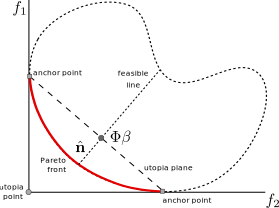
\includegraphics[width=0.8\columnwidth]{Ch5NBI}%
	\caption{\gls{nbi} optimization method.}%
	\label{fig:NBI}%
\end{figure}
%
figure~\ref{fig:NBI}, a representation of the method is shown for two normalized objective functions. If the utopia plane (the plane that contains the anchor points, in the case of a bi-objective problem, the straight line that joins the anchor points) is parameterized by $\Phi\mathbf{\beta}$, where $\Phi(:,i)=\mathbf{F}(\mathbf{x}_i^*)-\mathbf{F}(\mathbf{x}^*)$, $\mathbf{F}(\mathbf{x}_i^*)$ is the value of the multi-objective function evaluated in the $i$th anchor point, $\mathbf{F}(\mathbf{x}^*)$ is the value of the function at the utopia point, and $\beta$ is chosen as:
\begin{equation}
\beta=
\left[\begin{tabular}{c}
$\alpha_{1NBI}$ \\ $\alpha_{2NBI}$
\end{tabular}\right],
\label{eq:Beta}
\end{equation}
with $\alpha_{1NBI}+\alpha_{2NBI}=1$.

The central idea behind the \gls{nbi} method is to find the maximum distance from the utopia plane towards the utopia point (with direction $\hat{\mathbf{n}}$) that is normal (or quasi normal as proposed in \citet{Das1998}) to the utopia plane. In other words, this method finds the border of the feasible region that is closer to the utopia point (farther from the utopia plane). This problem is considered a subproblem, because with one given $\beta$,only one point of the Pareto front is found but, by varying this parameter $\beta$ evenly, it is possible to obtain an even spaced realization of the front.

The problem then is posed as follows:%
%
\begin{equation}
\begin{gathered}
\max_{\xv,v}{\;v}, \\
\text{s.t.} \ \Phi \boldsymbol{\beta} + v \hat{\mathbf{n}} = \mathbf{F}(\xv),\\
h(\xv)=0, \\
g(\xv) \leq 0.
\end{gathered}
\label{eq:NBIProblem}
\end{equation}%

The \gls{nbi} method converts the original problem by adding an equality constraint. By maximizing the new variable $v$ (which represents the distance from the utopia plane towards the utopia point), the front that is closer to the utopia point is found. An alternative formulation of \eqref{eq:NBIProblem} was proposed in \citet{Shukla2007} to ensure that only the points that really belongs to the Pareto front are found.

This method has been widely used in several areas.For example, in \citet{Stehr2003} was used to analyze the compromise between gain and phase margin when designing analog circuits. In \citet{Sendin2004}, the \gls{nbi} was considered in the design of nonlinear bioprocesses. In \citet{Ierapetritou2007a} the \gls{nbi} is used to optimize the scheduling of a chemical process with uncertainty. In \citet{Vahidinasab2010} \gls{nbi} is applied to develop optimal bidding strategies for the participants of oligopolistic energy markets; the social welfare and the emissions are considered as the cost functions and the constraints take into account the characteristics of the generators and the power flow of the system. In \citet{Ganesan2013}, \gls{nbi} is used in conjunction with a meta-heuristic algorithm to generate optimal solution options to the green sand mould system problem. In \citet{Brito2014} the method is used coupled with mean-squared error functions in a robust parameter design of the surface roughness in end milling process. In \citet{Rubio-Largo2014} the method is adapted to solve a traffic grooming problem in the telecommunication field. In \citet{Rojas2015b} a comparison between several scalarization methods, including \gls{nbi}, was presented for a \gls{foptd} plant where different disturbance sources are considered. In \citet{Naves2017} \gls{nbi} is used for the optimization of methyl orange treatment with ozone. In \citet{Simab2018} a model for short-term hydrothermal scheduling problem in the presence of the pumped-storage technology and stated as Mixed-Integer Non-Linear Programming, while the scalarization was done using \gls{nbi}. Finally, in \citet{Moura2018} \gls{nbi} was used in the construction of a Pareto boundary chart of a treatment of a synthetic solution of amoxicillin in a reactor with ozone bubbling.
%-------------------------------------------------- 
\subsection{Normalized Normal Constraint}
\label{sec:NNC}
The \gls{nnc} is presented in \citet{Messac2003} and is intended to improve the results of the \gls{nbi} by formulating the optimization problem only with inequality constraints and by filtering all the non-Pareto optimal points. The main idea of the methodology is presented in
%
\begin{figure}[b]%
	\centering
	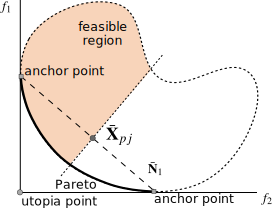
\includegraphics[width=0.8\columnwidth]{Ch5NNC}%
	\caption{NNC optimization method.}%
	\label{fig:NNC}%
\end{figure}
%
figure~\ref{fig:NNC}: the utopia plane is parameterized in a similar way as the \gls{nbi} but, instead of constraining the points to be within a line, the new constrained feasible region is constructed with the original feasible region and a line that is normal to the utopia plane. With this new feasible region it is only required to minimize one of the functions (e.g. $f_{1}$) in order to find the Pareto front.

By varying the parameter $\bar{\mathbf{X}}_{pj}$ along the utopia plane, it is possible to find an even spaced front. $\bar{\mathbf{X}}_{pj}$ is computed as%
%
\begin{equation}
\bar{\mathbf{X}}_{pj}= \alpha_{1NNC} \mathbf{\hat{F}}(\mathbf{x}_1^*)+\alpha_{2NNC} \mathbf{\hat{F}}(\mathbf{x}_2^*).
\label{eq:Xpj}
\end{equation}%
%
with $\alpha_{1NNC}+\alpha_{2NNC}=1$ and where $\mathbf{\hat{F}}(\mathbf{x}_1^*)$ is the first anchor point and $\mathbf{\hat{F}}(\mathbf{x}_2^*)$ is the second. The methodology can be extended to higher dimensions.

The optimization problem can be written as follows:
%
\begin{equation}
\begin{gathered}
\min_{\mathbf{x}}{\; \hat{f}_{1}(\mathbf{x})}, \\
\text{s.t.} \ \bar{\mathbf{N}}_1^T \left(\hat{\mathbf{F}}(\mathbf{x})-\bar{\mathbf{X}}_{pj}\right) \leq 0,\\
h(\mathbf{x})=0, \\
g(\mathbf{x}) \leq 0,
\end{gathered}
\label{eq:NNCProblem}
\end{equation}
%
where $\bar{\mathbf{N}}_1$ is the vector that contains the direction of the utopia plane. In some cases, the optimization may yield points that do not belong to the Pareto front. In \citet{Messac2003}, the authors propose to use a filter algorithm to eliminate those points.

This method has been used in several cases. Also in \citet{Hosseini2016a} the method was implemented to optimally solve the transmission congestion management taking into account the cost of congestion management, voltage stability margin, and transient stability margin. In \citet{Sanchez2017a}, the \gls{nnc} was considered to find optimally balanced tuning rules for fractional-order proportional-integral-derivative controllers for \gls{foptd} process models subject to a robustness constraint. In \citet{Mittal2017a} the NNC was used in conjunction with an evolutionary algorithm to find the optimum number and location of wind turbines in a wind farm. In \citet{Benki2018}, the \gls{nnc} was implemented in the design of an aerosol can, tanking into account both the dome growth and the dome reversal pressure DRP. In \citet{Tan2018a}, the \gls{nnc} was applied in the design of microvascular panels for battery cooling applications. The NNC is also applied in \citet{Liu2019} within their algorithm to optimally control the glycerol in a 1,3-propanediol batch process.

\subsection{Enhanced Normalized Normal Constraint}
\label{sec:ENNC}
The \gls{ennc} \citet{Sanchis2008}, is a new perspective of the original \gls{nnc} method. Implicitly, the \gls{nnc} method supposes that in each anchor point, the other functions that are not optimal, have their worst value. For a two functions optimization, this is always the case; however for more than two functions this supposition is not true in general. The \gls{ennc} method redefines the anchor points in such a way that the supposition of the \gls{nnc} holds true, and then the same method may be used. Other advantage of the \gls{ennc} is that it is possible to expand the explored regions of the problem, given a better representation of the Pareto front.
%
The new anchor points (called pseudo anchor points) are defined as:
\begin{equation}
F_i^{**} = \left[
\begin{tabular}{cccccc}
$f_1^N$ & $f_2^N$ & $\cdots$ & $f_i^{*}$ & $\cdots$ & $f_n^N$
\end{tabular}
\right],
\label{eq:PseudoAnchor}
\end{equation}
%
where $f_i^N$ if the value of function $f_i$ at the pseudo nadir point. The effect of this new definition is to enlarge the utopia hyper plane and scaling the functions in such a way that the Pareto front is evenly obtained while the unexplored regions of the Pareto are reduced.

The Pareto is then computed using the same methodology as in the \gls{nnc} case. This method has also been applied in several cases, for example in \citet{Contreras-Leiva2016}, the \gls{ennc} is applied in the optimization of the tuning parameters of a \gls{2dof} \gls{pid} controller for an \gls{soptd} plant. In\citet{Pereira2017b} an augmented version of the \gls{ennc} is applied to optimized the milling process of aluminum alloy Al 7075 taking into account the axial cutting force, the energy consumption and the material removal rate. The \gls{ennc} is tested in the optimization of a multiobjective model based predictive controller and compared with different techniques in \citet{Toro2011} and for the nonlinear case in \citet{Vallerio2014}.
%--------------------------------------------------
\section{Solution selection from the Pareto front}
\label{sec:Selection}
%%--------------------------------------------------------------------------
%%-------------------------------o-o-o--------------------------------------
%%--------------------------------------------------------------------------
The optimizations techniques presented in Section~\ref{sec:design-methodologies} are very well suited to find the Pareto Front of a multiobjective optimization problem. However, in the end, it is necessary to decide which of the multiple equally optimal points is the one that is going to be selected as the final solution.

Consider the general Pareto Front presented in 
\begin{figure}[b]
	\centering
	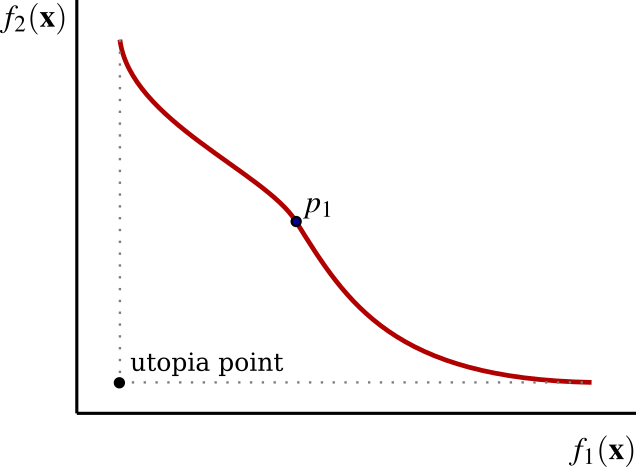
\includegraphics[width=0.8\columnwidth]{Ch5GeneralPareto}
	\caption{General Pareto Front with one solution selected.}
	\label{fig:Ch5GeneralPareto}
\end{figure}
%
Figure~\ref{fig:Ch5GeneralPareto}. Once the Pareto is computed, it is certainly very useful to plot it to see how the cost functions $f_1(\mathbf{x})$ and $f_2(\mathbf{x})$ vary with the change in the decision variables $\mathbf{x}$. In this figure, the arbitrary solution $p_1$ is pointed out. By definition, all points in the Pareto Front are equally optimal, therefore, what makes $p_1$ any special from other points? More important, how any of the Pareto points can be selected from any other?

One may then conclude that obtaining the Pareto front is half the solution to the \gls{moop}. The final task to fully solve the problem is to be able to select one of the (maybe infinite) possible points of the Pareto. With a front like the one presented in Figure~\ref{fig:Ch5GeneralPareto}, it may be easy to explore all possible solutions, but with more than three objective functions, it is impossible to directly plot the front. And even with three objectives, the visualization of the results may be cumbersome.

Even more, the plot of Figure~\ref{fig:Ch5GeneralPareto} contains the solutions viewed from the function space, but what is really necessary is to know the value of the decision variables. But each of every point in the Pareto is associated with a $n$-size vector representing one of the optimal solutions. Once again, plotting the Pareto is not enough to help the decision maker to solve the problem.

For these reasons, once the Pareto is found, it may be useful to accomplish some tasks to help the decision maker:
\begin{itemize}
	\item  Visualize the Pareto to understand the relation between the cost functions and the decision variables.
	\item Use the Pareto as data for the construction of a decision tool.
	\item Use the Pareto as part of a decision tool.
\end{itemize}
In the following, these three tasks are going to be explored.
%
\subsection{Visualization of the Pareto Front}
\label{sec:ParetoVisualization}
%
One of the advantages of using a multiobjective problem approach, is its ability to take into account many cost functions at the same time, and being able to find the set of the \emph{best} solutions. This is the ultimate goal of a multiobjective optimisation, to provide useful information to the decision makers in order to help to choose according to its preferences. This can be done in terms of a large set of raw data that has lately to be processed accordingly. This introduces some cognitive issues that become harder and a clear obstacle for decision making stage, especially when having many objectives (say more than 3). Although there are some performance metrics that can evaluate the quality of a Pareto front approximation set (Inverted Generational Distance \citep{Bosman2003} and Hypervolume \citep{Zitzler1999} among others), it is still not intuitive this approach really helps the decision maker to understand the trade-off relationship among objectives.

In contrast, high-dimensional data visualisation is a widely recognised effective way to facilitate the analysis and understanding of multidimensional data. more effective and intuitive to facilitate the decision maker stage to understand the trade-off solutions and thus make a meaningful decision. In the context of multi-objective optimisation, comparing to quantitative performance metrics, visualisation is, in principle, able to provide a decision maker better insights about Pareto front approximation sets (e.g. the distribution of solutions, the geometric characteristics of Pareto front approximation) thus to facilitate the decision-making (e.g. the exploration of trade-off relationship, the knee region or region of interest).

According to \citet{Gao2019} a high quality visualisation tool must provide three types of information in the high dimensional space. 
\begin{itemize}
\item  Should provide accurate shape, location, and range of the approximate Pareto front. 
\item  From the provided visualisation, decision makers can observe trade-off between objectives, monitor the evolution progress, assess the quality of the approximate front, and select their preferred solutions if desired. 
\item  Should be scalable to any dimensions, handle a large number of individuals on the approximate front, and simultaneously visualise multiple fronts for the purpose of visual comparison. Moreover, the resulted visualisation plot should be robust and insensitive to the addition or removal of an individual.
\end{itemize}

To tackle these issues, different kinds of plots have been proposed in the literature that tries to present all the information of the Pareto in a bi-dimensional graph. Generally speaking, they can be divided into three categories. Interested readers are encouraged to found a recent taxonomy from \citet{B.2018}.

\begin{description}
\item [A. Visualisation of All Objective Information] These visualisation techniques aim to reveal all individual objective information of the underlying approximation set. Specifically, scatter plot is the most commonly utilised data visualisation technique that provides a holistic exploration of the population distribution. 

\item [B. Visualisation via Dimension Reduction] Techniques in this category aims to transform the high-dimensional data into a lower dimensional space to facilitate the human cognition. In modern data analytics, there are many dimension reduction techniques available to implement such transformation.  Instead of using dimension reduction techniques from machine learning, In \citet{Blasco2008}, Blasco et al. proposed a new visualisation technique called level diagrams to visualise the approximation set in a objective-wise manner. More specifically, each diagram is a two-dimensional scatter plot where the horizontal coordinate represents the objective value at the corresponding objective while the vertical coordinate indicates the distance with respect to the ideal point. As claimed by the authors, the level diagrams are able to facilitate the investigation of some of the Pareto front characteristics, i.e. discontinuities, closeness to ideal point and ranges of attainable values. 

\item [C. Visualisation via a Transformed Coordinate System] Techniques in this category share some similarity with the dimension reduction. They also aim to visualise the original high-dimensional data in a lower-dimensional space. But they try to maintain the original information as much as possible. For example, Ibrahim et al. \citet{Ibrahim2016} developed a variant of the classic Radial coordinate visualisation (RadViz) \citep{Hoffman2002}, called 3D-RadViz, by adding an additional dimension. In particular, this additional dimension represents the perpendicular distance between a solution and a hyper-plane formed by the extreme points of the underlying population. By doing so, the 3D-RadViz is able to provide the information of the convergence of the population. 
\end{description}

As usual when there do exist different approaches to deal with a complex problem, there is  no single visualisation technique is able to provide a comprehensive understanding of the characteristics of the approximation set. It is important to know the specific characteristics, pros and cons of each approach and evaluate the suitability for the problem at hand.
  
\subsection{The Pareto as a decision tool}
\label{sec:ParetoData}
%
Since the Pareto front cannot be considered as the final solution of the \gls{moop}, one may use it as the basis to construct a tool that takes advantage of the multiple optimal points found.

In other words, the Pareto front becomes the raw material that is used to produce the final decision tool. This tool may be an algorithm (as a tuning rule for PID controllers for example) that incorporates the information obtained from the optimization to produce a final decision.

For example in \cite{Zhao2007}	the concept of Pareto optimality is used to define a genetic programming approach for optimal decision trees. The author presented a Java code for the final tool and use code in two different study cases.

Another example can be found in \cite{Das2012}. In this paper, the route for the transportation of hardzarous waste has to be selected taking into account the cost of the route and the mortality and morbidity of incidents. Once the Pareto frontier has been obtained, the authors present a selection criteria where the Cost Elasticity of risk and the Knees on the Pareto are taken into account for the final decision.
%
%\subsection{The Pareto Front as part of a decision tool}
%\label{sec:ParetoDecision}
%\textbf{To do}
%
\bibliographystyle{spbasic}
\bibliography{ReferenciasMulti}